\chapter{Evaporative purification}
\graphicspath{{./evaporation/graphs/}}

In order to study the effects of $N$, the first thing needed is to obtain monodisperse samples with different $N$ values. This has been achieved through evaporative purification technique, which has been practiced on low molecular weight polystyrene, and proved to be an efficient way to obtain highly monodisperse polymers \cite{Zhu2017a}.

\section{Vapor pressure of PEO oligomers}

For a particular polymer, as its $N$ decreases, its vapor pressure increases, and for polymers with small enough $N$ values, their vapor pressure could be significant at high temperatures (lower than their thermal degradation temperature). This fact potentially allows one to separate polymer components with different $N$ values, by applying an evaporation method with the similar idea of distillation.

To examine the feasibility of separating components through evaporation, it is a good idea to first look at their vapor pressures. Unfortunately, there are few data of vapor pressure of pure PEO \cite{Krieger2018}, either from calculation or experimental measurements. Therefore, we applied a theoretical model to calculate the vapor pressures of low molecular weight PEO.

Sanchez and Lacombe Lattice-Fluid Model \cite{Sanchez1976} describes a fluid using only three molecular parameters, and provides a method to calculate the relation between vapor pressure and temperature for a given $N$ value. These three parameters for PEO could be found in the literature \cite{Rodgers1993}.

In this model, Gibbs free energy G is a function of mass density $\rho$:

\begin{equation}
G = - \rho + P\nu + T[(\nu - 1)\ln(1 - \rho) + \dfrac{1}{r}\ln(\rho/\omega)]  \label{eqn_Gvsrho}
\end{equation}

\noindent
where $\rho$ is density, $P$ is pressure, $\nu$ is volume, $T$ is temperature, $r$ is the number of monomers in a polymer molecule, and $\omega = \delta r/\sigma e^{r-1}$. For a specific $N$ at given pressure and temperature, G could be plotted as a function of $\rho$ as shown below.

\begin{figure}[H]
\center
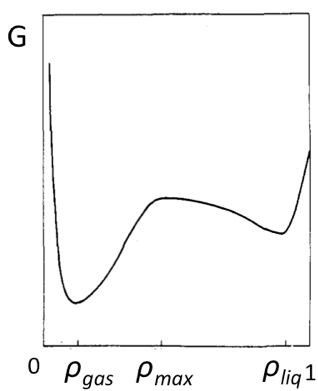
\includegraphics[width=0.3\linewidth]{Gvsrho}
\caption[Gibbs free energy vs mass density, where a liquid phase is metastable with respect to the vapor phase]{Gibbs free energy vs mass density, where a liquid phase is metastable with respect to the vapor phase \cite{Sanchez1976}.}
\label{fig:Gvsrho}
\end{figure}

The curve has two local minima. The first minimum represents gas phase, with lower mass density, and the second minimum represents liquid phase, with higher mass density. By tuning pressure or temperature, the two minima could be adjusted to be equal. This means the system has equal probability to be in the state of either gas or liquid. At a given temperature, there exists only one pressure that satisfies this equality, and this pressure and temperature are defined as the saturation pressure and temperature. The locus of all the saturation points represents the saturation/coexistence line, which is in fact the curve of vapor pressure as a function of temperature.

Solving for Equation \ref{eqn_Gvsrho} and applying the three molecular parameters found in literature, we were able to calculate the vapor pressure curve for each $N$ value of PEO oligomers. The results are shown in the plot below, and note that each curve has been generated from 10-20 data points.

\begin{figure}[H]
\center
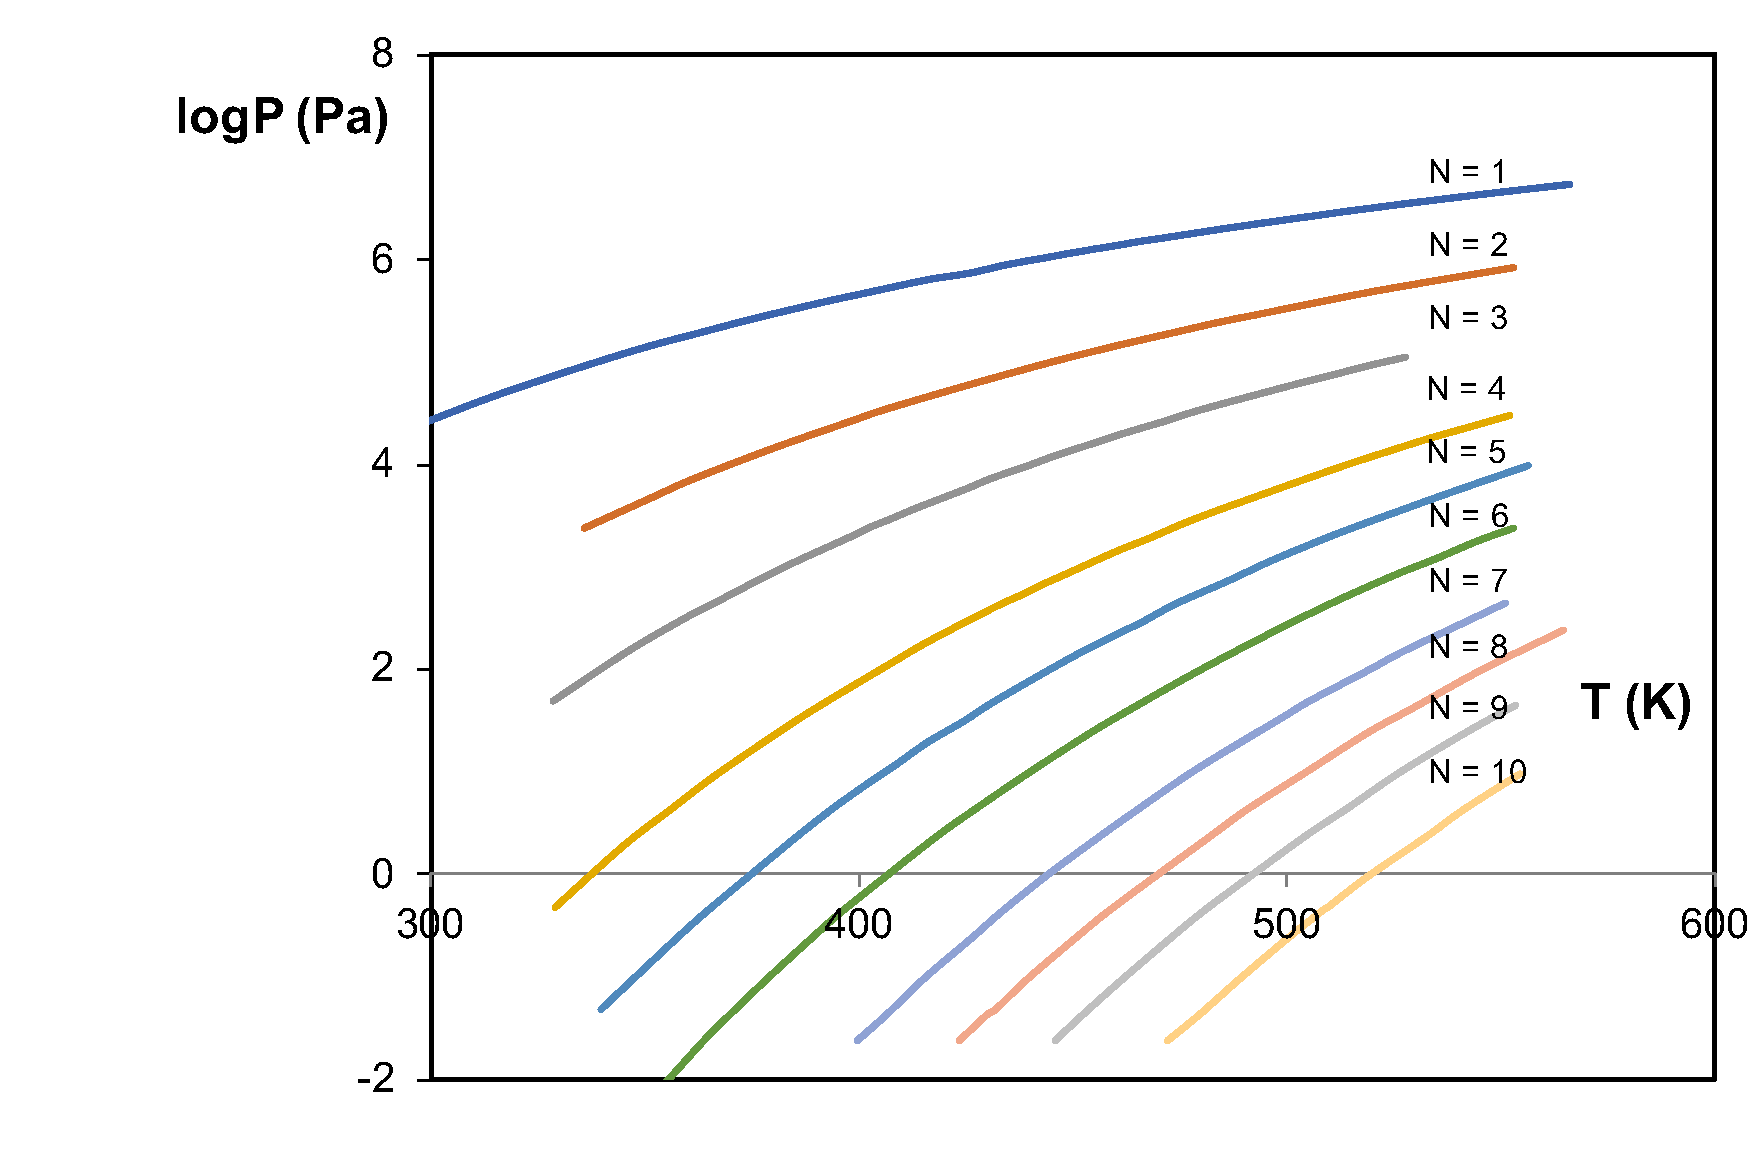
\includegraphics[width=\linewidth]{PvsT}
\caption{Plot of vapor pressure vs temperature for PEO oligomers with $N$ values from 1 to 10.}
\label{fig:VPvsT}
\end{figure}

The results for vapor pressures calculated from this model are not expected to be numerically correct, but they provides a good guidance in terms of the trend of vapor pressure curves and the gaps between neighboring N's. For a specific N, vapor pressure increases with temperature; for a specific temperature, vapor pressure decreases with N. More importantly, at a given temperature, the vapor pressures of two neighboring N's have a difference up to two orders of magnitude. However, this difference gets smaller as temperature goes higher, which indicates that it would be increasingly difficult to achieve a neat separation, and the purification products are expected to be more polydisperse under higher evaporation temperature. Evaporation temperature should never get close to 533K \cite{Choukourov2009}, which is the critical temperature where PEO starts thermal degradation in vacuum.

\section{Evaporation technique and results}

The experimental setup for evaporative purification is generally the same as the setup used for polystyrene \cite{Zhu2017a}. 96 mg of neat PEO 600 sample is placed on top of a polished silicon wafer of 2 cm $\times$ 2 cm in size and 0.3 mm in thickness. Si wafer acts as a bottom substrate and is placed onto a Linkam hot stage in a home-built vacuum chamber. In order to collect depositing fractions, another Si wafer of 5 cm $\times$ 5 cm in size is held approximately 3 mm right above the neat material, by thermal insulating spacers.

Before the beginning of each evaporation period, the chamber is pumped down with a dry scroll pump to an initial pressure of around 0.3 mbar. After that, we flush the chamber with nitrogen, and then evacuate it again. This process is repeated several times to flush out oxygen in the chamber, so to prevent the oxidation of polymer. Three time of flushing leads to an oxygen level of approximately $4.7 \times 10^{-6}$ times the oxygen level in atomsphere. %calculated using -29.5 inhg lower than asmosphere.
Finally, we introduce a small amount of nitrogen into the chamber, until the pressure is raised to about 170 mbar. The reason for this action is because during the evaporation, the system requires a good thermal conduction to drive away excess heat from the hot stage, so to maintain a stable temperature (with a fluctuation of less than 1K) of the material.

We start the evaporation from 393K, and the evaporated material is collected every two hours. Products from the first four hours are not collected, as they may contain impurities such as initiators. We seal the product from each period into an aluminum sample pan, in preparation for future differential scanning calorimetry measurements and mass spectroscopy measurements.

Figure \ref{fig:massvstime} shows that within each temperature region during the evaporation, the mass of material collected experiences a general decreasing trend, and the mass of products collected into sample pans ranges from 0.2 mg to 2.9 mg. We expected that each temperature region would correspond to a majority of a specific N, so the sample gets purified.

\begin{figure}[H]
\center
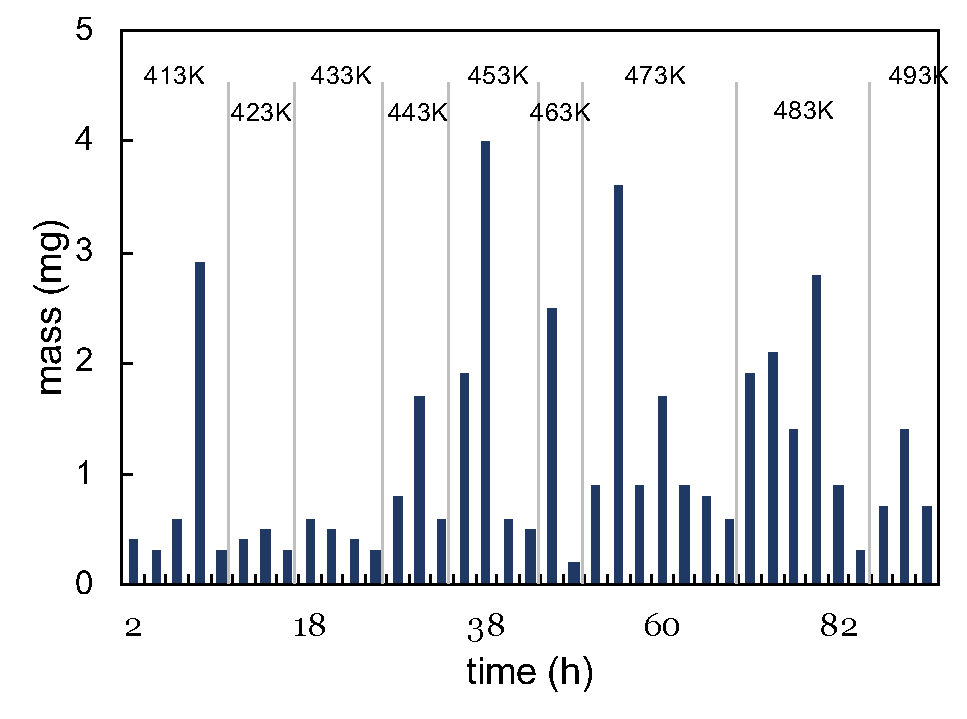
\includegraphics[width=0.8\linewidth]{massvstime}
\caption{Mass of PEO collected with respect to time and temperature.}
\label{fig:massvstime}
\end{figure}

\section{Results from mass spectroscopy}

To obtain information about the actual distribution of different N's in each fraction, mass spectroscopy measurements are performed on several samples. Matrix Assisted Laser Desorption/Ionization – time of flight (MALDI-TOF) technique was applied, with a Bruker Autoflex Speed MALDI-TOF mass spectrometer to conduct the measurements.

A typical MALDI-TOF mass spectroscopy works with the following procedure:

\begin{itemize}
\item Mix the analyte (polymer sample in our case) with appropriate matrix material.
\item Bombard the mixed material with laser, and the laser energy is absorbed by the matrix, which get desorbed and ionized, and a phase transition from solid to gas takes place in the matrix material.
\item A hot plume is generated, and during the flight of both the matrix material and the analyte, collisions among particles could result in the ionization of the analyte.
\item Ions flying into the the TOF mass spectrometer are separated due to different mass (m)-to-charge (z) ratios. With the same kinetic energy, lighter ions arrive at the detector earlier than heavier ions.
\end{itemize}

From the spectrum generated, we are able to obtain information about the exact distribution of molecular weights, from which $M_{n}$, $M_{w}$, and PDI can be calculated.

\subsection{MALDI-TOF spectra and analysis}

MALDI measurements were carried out for 10 samples out of all the fractions, the neat PEO sample, and the leftover sample after all the evaporation periods. Figure \ref{fig:MALDIfractions} compares the purified fractions and shows the changes in molecular weight distribution during the evaporation process, with the green background spectrum being the neat sample.

\begin{figure}[H]
\center
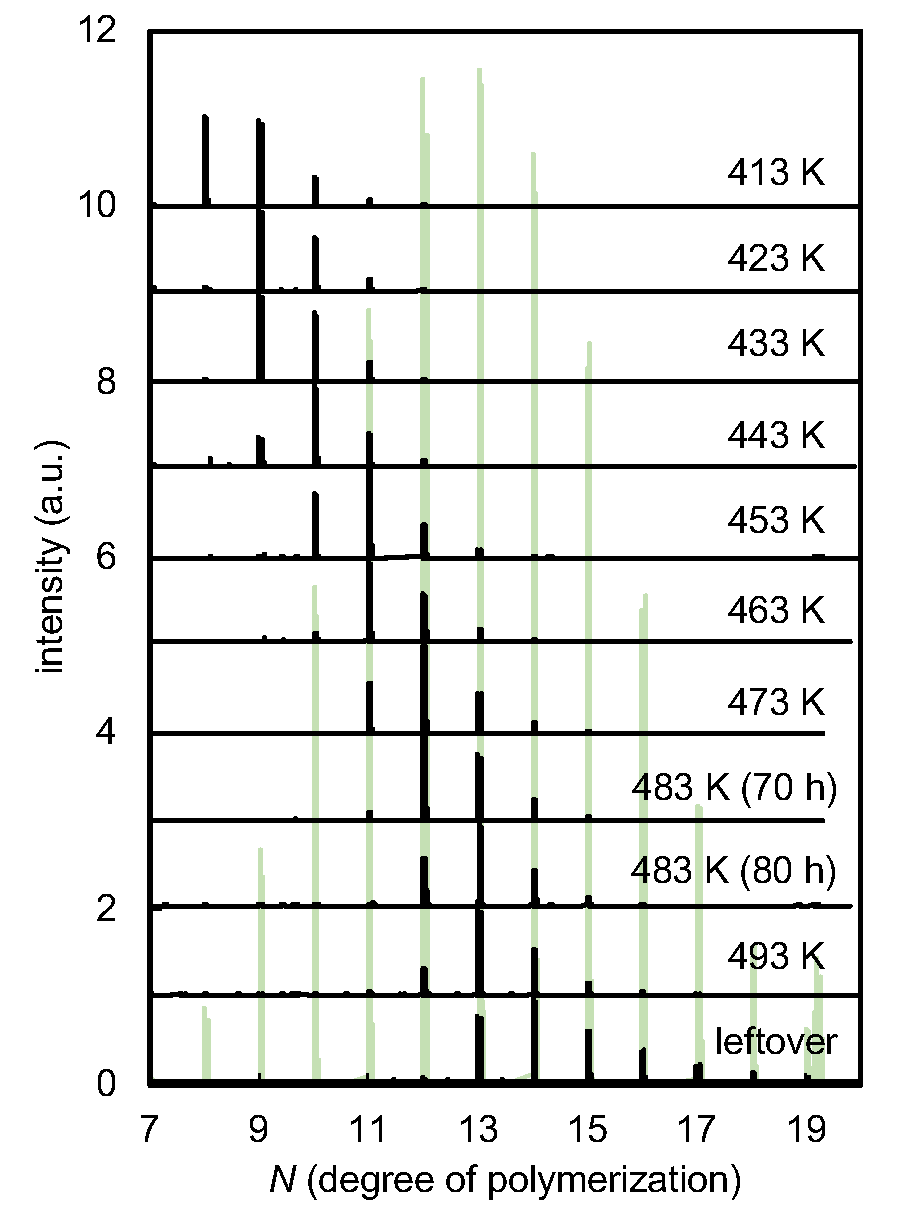
\includegraphics[width=0.6\linewidth]{MALDIfractions}
\caption{MALDI spectra of purified products (black) and neat sample (green) (80 h: 80th hour since start of evaporation).}
\label{fig:MALDIfractions}
\end{figure}

As the evaporation temperature increases, the $N$ values composing of each fraction shift towards higher values, ranging from 8 to 16. With the intensity of each peak, we are able to calculate their $M_{n}$, $M_{w}$, and PDI, and make quantitative comparisons. Compared to the neat sample, the spectra of the products are much narrower, meaning they are highly monodisperse. The lowest PDI we achieved is calculated to be 1.0052, and $(PDI - 1)$ is around six times better compared to 1.0306 of the neat sample.

\begin{figure}[H]
\center
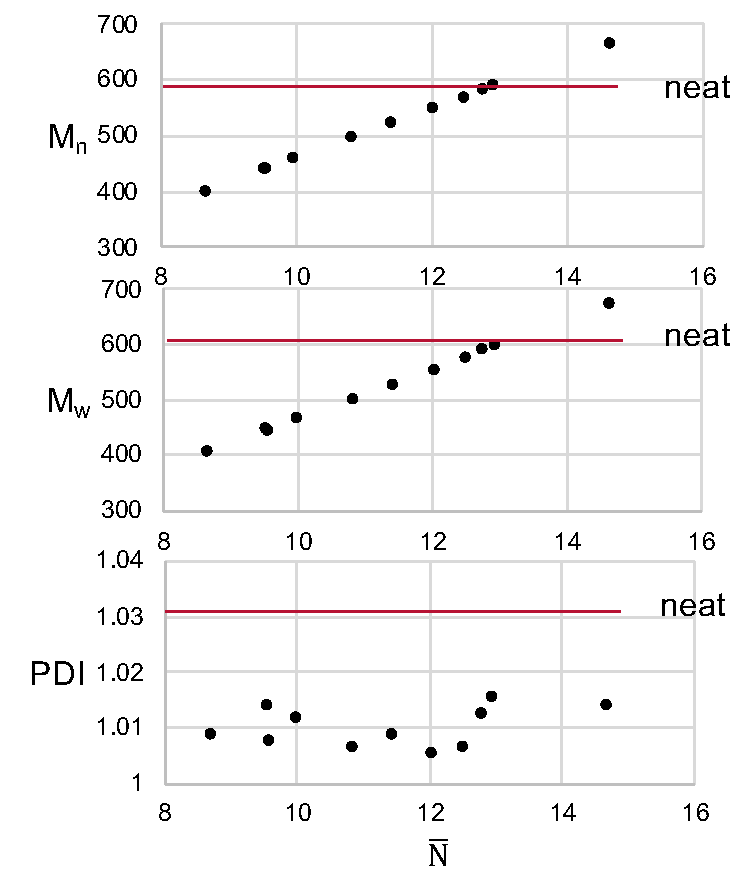
\includegraphics[width=0.6\linewidth]{fromMALDI}
\caption{$M_{n}$, $M_{w}$, and PDI comparison between products and neat sample.}
\label{fig:fromMALDI}
\end{figure}

\subsection{Evolution of $N$ during evaporation process}

So far we know the distribution of $N$'s at these 10 points during evaporation. However, it would be ideal if we could generate the evolution of $N$ values at any point without doing MALDI measurements on every single sample. In order to achieve this, we first plot the evolution of each $N$ value as a function of evaporation time, based on the percentage fraction of each $N$ in the products from different points during the evaporation process. Then we fit the ten data points for each $N$ value with Gaussian curves, which enables us to estimate the distribution of all $N$'s at any point during the evaporation (by applying interpolation only) (Figure \ref{fig:Nevolution}).

\begin{figure}[H]
  \centering
  \begin{subfigure}[b]{0.6\linewidth}
    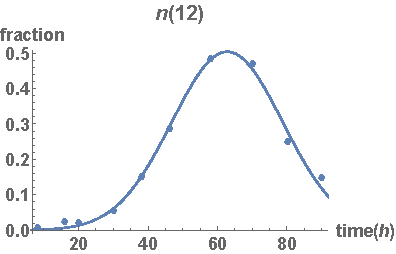
\includegraphics[width=\linewidth]{fitN12}
    \caption{Percentage fraction of $N$ = 12 in samples from different evaporation time.}
    \vspace{1 cm}
  \end{subfigure}
  \begin{subfigure}[b]{0.6\linewidth}
    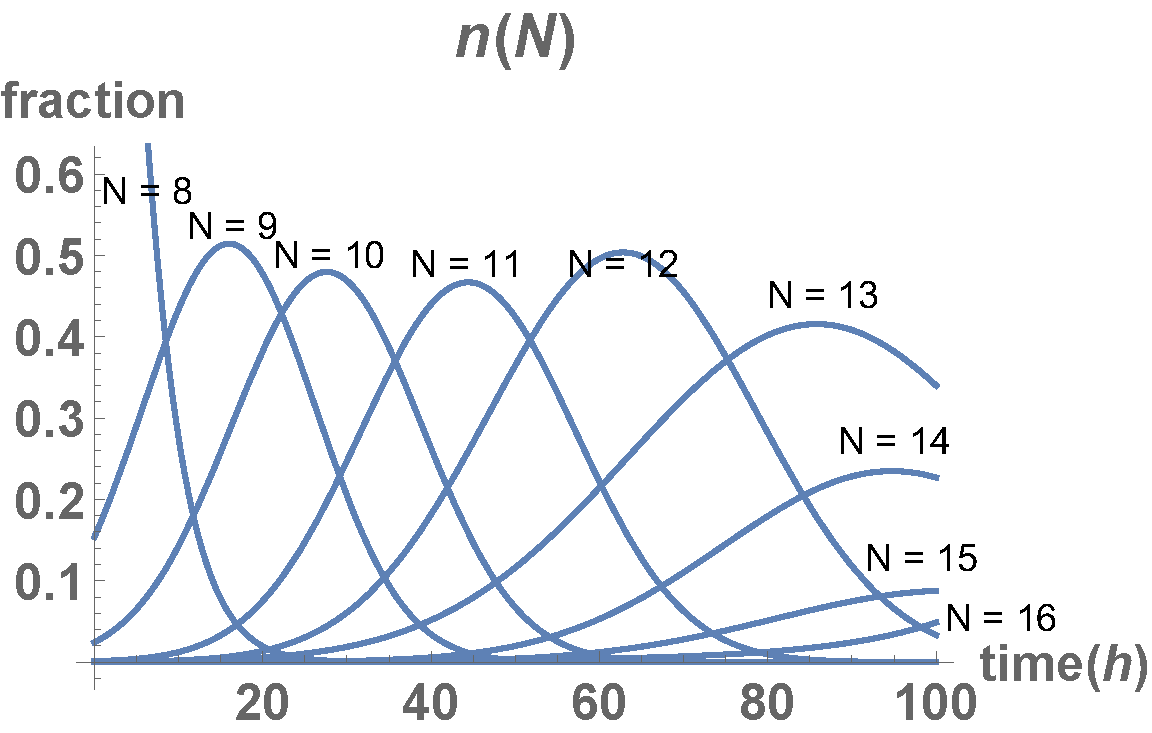
\includegraphics[width=\linewidth]{fitallNs}
    \caption{Evolution of $N$ values (from 8 to 16).}
  \end{subfigure}
  \caption{Evolution of $N$ values during evaporation process.}
  \label{fig:Nevolution}
\end{figure}